%!TeX root=../emmatop.tex
\chapter[Chapter \thechapter]{}
	
\lettrine[lraise=0.3,ante=`]{I}{} hope I shall soon have the pleasure of introducing my son to you,' said Mr Weston.

\zz
Mrs Elton, very willing to suppose a particular compliment intended her by such a hope, smiled most graciously.

<You have heard of a certain Frank Churchill, I presume,> he continued—<and know him to be my son, though he does not bear my name.>

<Oh! yes, and I shall be very happy in his acquaintance. I am sure Mr Elton will lose no time in calling on him; and we shall both have great pleasure in seeing him at the Vicarage.>

<You are very obliging.—Frank will be extremely happy, I am sure.— He is to be in town next week, if not sooner. We have notice of it in a letter to-day. I met the letters in my way this morning, and seeing my son's hand, presumed to open it—though it was not directed to me—it was to Mrs Weston. She is his principal correspondent, I assure you. I hardly ever get a letter.>

<And so you absolutely opened what was directed to her! Oh! Mr Weston—(laughing affectedly) I must protest against that.—A most dangerous precedent indeed!—I beg you will not let your neighbours follow your example.—Upon my word, if this is what I am to expect, we married women must begin to exert ourselves!—Oh! Mr Weston, I could not have believed it of you!>

<Aye, we men are sad fellows. You must take care of yourself, Mrs Elton.—This letter tells us—it is a short letter—written in a hurry, merely to give us notice—it tells us that they are all coming up to town directly, on Mrs Churchill's account—she has not been well the whole winter, and thinks Enscombe too cold for her—so they are all to move southward without loss of time.>

<Indeed!—from Yorkshire, I think. Enscombe is in Yorkshire?>

<Yes, they are about one hundred and ninety miles from London, a considerable journey.>

\begin{figure}[tbph]
\centering
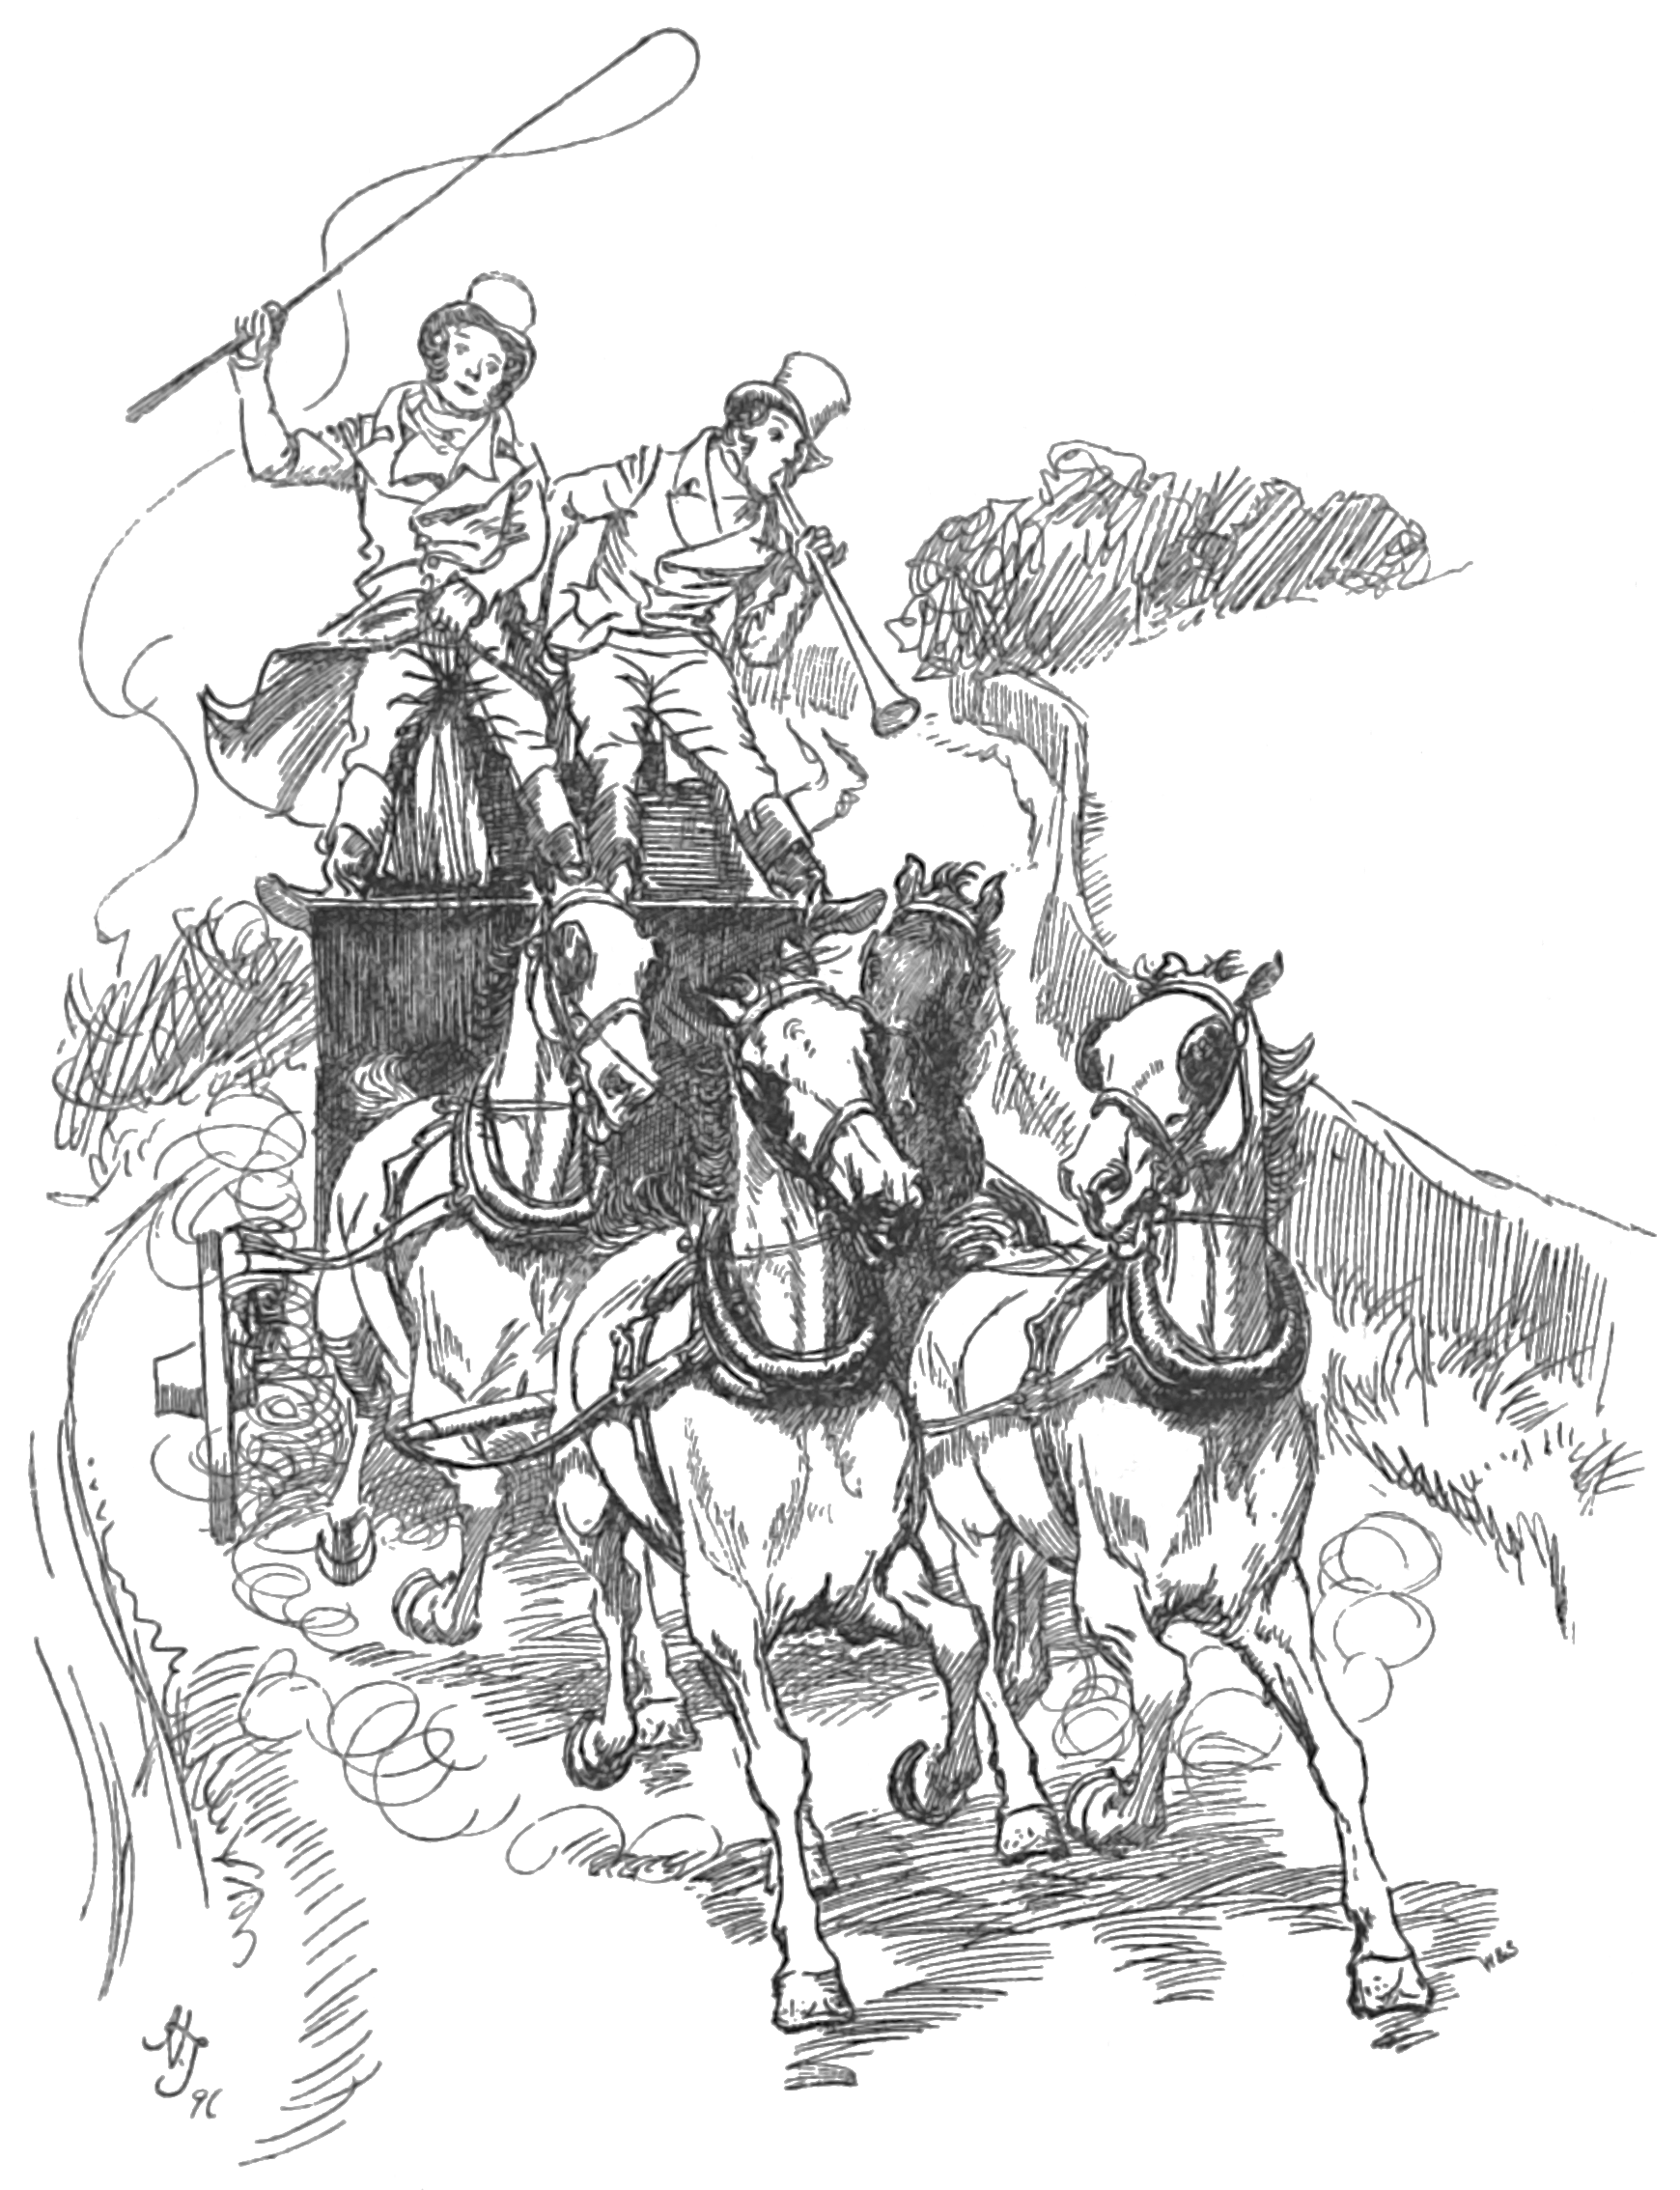
\includegraphics[width=.9\linewidth]{36flies}
\caption{<How my brother, Mr Suckling, sometimes flies about>}
\end{figure}

<Yes, upon my word, very considerable. Sixty-five miles farther than from Maple Grove to London. But what is distance, Mr Weston, to people of large fortune?—You would be amazed to hear how my brother, Mr Suckling, sometimes flies about. You will hardly believe me—but twice in one week he and Mr Bragge went to London and back again with four horses.>

<The evil of the distance from Enscombe,> said Mr Weston, <is, that Mrs Churchill, as we understand, has not been able to leave the sofa for a week together. In Frank's last letter she complained, he said, of being too weak to get into her conservatory without having both his arm and his uncle's! This, you know, speaks a great degree of weakness—but now she is so impatient to be in town, that she means to sleep only two nights on the road.—So Frank writes word. Certainly, delicate ladies have very extraordinary constitutions, Mrs Elton. You must grant me that.>

<No, indeed, I shall grant you nothing. I always take the part of my own sex. I do indeed. I give you notice—You will find me a formidable antagonist on that point. I always stand up for women—and I assure you, if you knew how Selina feels with respect to sleeping at an inn, you would not wonder at Mrs Churchill's making incredible exertions to avoid it. Selina says it is quite horror to her—and I believe I have caught a little of her nicety. She always travels with her own sheets; an excellent precaution. Does Mrs Churchill do the same?>

<Depend upon it, Mrs Churchill does every thing that any other fine lady ever did. Mrs Churchill will not be second to any lady in the land for>—

Mrs Elton eagerly interposed with,

<Oh! Mr Weston, do not mistake me. Selina is no fine lady, I assure you. Do not run away with such an idea.>

<Is not she? Then she is no rule for Mrs Churchill, who is as thorough a fine lady as any body ever beheld.>

Mrs Elton began to think she had been wrong in disclaiming so warmly. It was by no means her object to have it believed that her sister was not a fine lady; perhaps there was want of spirit in the pretence of it;—and she was considering in what way she had best retract, when Mr Weston went on.

<Mrs Churchill is not much in my good graces, as you may suspect—but this is quite between ourselves. She is very fond of Frank, and therefore I would not speak ill of her. Besides, she is out of health now; but that indeed, by her own account, she has always been. I would not say so to every body, Mrs Elton, but I have not much faith in Mrs Churchill's illness.>

<If she is really ill, why not go to Bath, Mr Weston?—To Bath, or to Clifton?> <She has taken it into her head that Enscombe is too cold for her. The fact is, I suppose, that she is tired of Enscombe. She has now been a longer time stationary there, than she ever was before, and she begins to want change. It is a retired place. A fine place, but very retired.>

<Aye—like Maple Grove, I dare say. Nothing can stand more retired from the road than Maple Grove. Such an immense plantation all round it! You seem shut out from every thing—in the most complete retirement.—And Mrs Churchill probably has not health or spirits like Selina to enjoy that sort of seclusion. Or, perhaps she may not have resources enough in herself to be qualified for a country life. I always say a woman cannot have too many resources—and I feel very thankful that I have so many myself as to be quite independent of society.>

<Frank was here in February for a fortnight.>

<So I remember to have heard. He will find an addition to the society of Highbury when he comes again; that is, if I may presume to call myself an addition. But perhaps he may never have heard of there being such a creature in the world.>

This was too loud a call for a compliment to be passed by, and Mr Weston, with a very good grace, immediately exclaimed,

<My dear madam! Nobody but yourself could imagine such a thing possible. Not heard of you!—I believe Mrs Weston's letters lately have been full of very little else than Mrs Elton.>

He had done his duty and could return to his son.

<When Frank left us,> continued he, <it was quite uncertain when we might see him again, which makes this day's news doubly welcome. It has been completely unexpected. That is, I always had a strong persuasion he would be here again soon, I was sure something favourable would turn up—but nobody believed me. He and Mrs Weston were both dreadfully desponding. <How could he contrive to come? And how could it be supposed that his uncle and aunt would spare him again?> and so forth—I always felt that something would happen in our favour; and so it has, you see. I have observed, Mrs Elton, in the course of my life, that if things are going untowardly one month, they are sure to mend the next.>

<Very true, Mr Weston, perfectly true. It is just what I used to say to a certain gentleman in company in the days of courtship, when, because things did not go quite right, did not proceed with all the rapidity which suited his feelings, he was apt to be in despair, and exclaim that he was sure at this rate it would be May before Hymen's saffron robe would be put on for us. Oh! the pains I have been at to dispel those gloomy ideas and give him cheerfuller views! The carriage—we had disappointments about the carriage;—one morning, I remember, he came to me quite in despair.>

She was stopped by a slight fit of coughing, and Mr Weston instantly seized the opportunity of going on.

<You were mentioning May. May is the very month which Mrs Churchill is ordered, or has ordered herself, to spend in some warmer place than Enscombe—in short, to spend in London; so that we have the agreeable prospect of frequent visits from Frank the whole spring—precisely the season of the year which one should have chosen for it: days almost at the longest; weather genial and pleasant, always inviting one out, and never too hot for exercise. When he was here before, we made the best of it; but there was a good deal of wet, damp, cheerless weather; there always is in February, you know, and we could not do half that we intended. Now will be the time. This will be complete enjoyment; and I do not know, Mrs Elton, whether the uncertainty of our meetings, the sort of constant expectation there will be of his coming in to-day or to-morrow, and at any hour, may not be more friendly to happiness than having him actually in the house. I think it is so. I think it is the state of mind which gives most spirit and delight. I hope you will be pleased with my son; but you must not expect a prodigy. He is generally thought a fine young man, but do not expect a prodigy. Mrs Weston's partiality for him is very great, and, as you may suppose, most gratifying to me. She thinks nobody equal to him.>

<And I assure you, Mr Weston, I have very little doubt that my opinion will be decidedly in his favour. I have heard so much in praise of Mr Frank Churchill.—At the same time it is fair to observe, that I am one of those who always judge for themselves, and are by no means implicitly guided by others. I give you notice that as I find your son, so I shall judge of him.—I am no flatterer.>

Mr Weston was musing.

<I hope,> said he presently, <I have not been severe upon poor Mrs Churchill. If she is ill I should be sorry to do her injustice; but there are some traits in her character which make it difficult for me to speak of her with the forbearance I could wish. You cannot be ignorant, Mrs Elton, of my connexion with the family, nor of the treatment I have met with; and, between ourselves, the whole blame of it is to be laid to her. She was the instigator. Frank's mother would never have been slighted as she was but for her. Mr Churchill has pride; but his pride is nothing to his wife's: his is a quiet, indolent, gentlemanlike sort of pride that would harm nobody, and only make himself a little helpless and tiresome; but her pride is arrogance and insolence! And what inclines one less to bear, she has no fair pretence of family or blood. She was nobody when he married her, barely the daughter of a gentleman; but ever since her being turned into a Churchill she has out-Churchill'd them all in high and mighty claims: but in herself, I assure you, she is an upstart.>

<Only think! well, that must be infinitely provoking! I have quite a horror of upstarts. Maple Grove has given me a thorough disgust to people of that sort; for there is a family in that neighbourhood who are such an annoyance to my brother and sister from the airs they give themselves! Your description of Mrs Churchill made me think of them directly. People of the name of Tupman, very lately settled there, and encumbered with many low connexions, but giving themselves immense airs, and expecting to be on a footing with the old established families. A year and a half is the very utmost that they can have lived at West Hall; and how they got their fortune nobody knows. They came from Birmingham, which is not a place to promise much, you know, Mr Weston. One has not great hopes from Birmingham. I always say there is something direful in the sound: but nothing more is positively known of the Tupmans, though a good many things I assure you are suspected; and yet by their manners they evidently think themselves equal even to my brother, Mr Suckling, who happens to be one of their nearest neighbours. It is infinitely too bad. Mr Suckling, who has been eleven years a resident at Maple Grove, and whose father had it before him—I believe, at least—I am almost sure that old Mr Suckling had completed the purchase before his death.>

They were interrupted. Tea was carrying round, and Mr Weston, having said all that he wanted, soon took the opportunity of walking away.

After tea, Mr and Mrs Weston, and Mr Elton sat down with Mr Woodhouse to cards. The remaining five were left to their own powers, and Emma doubted their getting on very well; for Mr Knightley seemed little disposed for conversation; Mrs Elton was wanting notice, which nobody had inclination to pay, and she was herself in a worry of spirits which would have made her prefer being silent.

Mr John Knightley proved more talkative than his brother. He was to leave them early the next day; and he soon began with—

<Well, Emma, I do not believe I have any thing more to say about the boys; but you have your sister's letter, and every thing is down at full length there we may be sure. My charge would be much more concise than her's, and probably not much in the same spirit; all that I have to recommend being comprised in, do not spoil them, and do not physic them.>

<I rather hope to satisfy you both,> said Emma, <for I shall do all in my power to make them happy, which will be enough for Isabella; and happiness must preclude false indulgence and physic.>

<And if you find them troublesome, you must send them home again.>

<That is very likely. You think so, do not you?>

<I hope I am aware that they may be too noisy for your father—or even may be some encumbrance to you, if your visiting engagements continue to increase as much as they have done lately.>

<Increase!>

<Certainly; you must be sensible that the last half-year has made a great difference in your way of life.>

<Difference! No indeed I am not.>

<There can be no doubt of your being much more engaged with company than you used to be. Witness this very time. Here am I come down for only one day, and you are engaged with a dinner-party!—When did it happen before, or any thing like it? Your neighbourhood is increasing, and you mix more with it. A little while ago, every letter to Isabella brought an account of fresh gaieties; dinners at Mr Cole's, or balls at the Crown. The difference which Randalls, Randalls alone makes in your goings-on, is very great.>

<Yes,> said his brother quickly, <it is Randalls that does it all.>

<Very well—and as Randalls, I suppose, is not likely to have less influence than heretofore, it strikes me as a possible thing, Emma, that Henry and John may be sometimes in the way. And if they are, I only beg you to send them home.>

<No,> cried Mr Knightley, <that need not be the consequence. Let them be sent to Donwell. I shall certainly be at leisure.>

<Upon my word,> exclaimed Emma, <you amuse me! I should like to know how many of all my numerous engagements take place without your being of the party; and why I am to be supposed in danger of wanting leisure to attend to the little boys. These amazing engagements of mine—what have they been? Dining once with the Coles—and having a ball talked of, which never took place. I can understand you—(nodding at Mr John Knightley)—your good fortune in meeting with so many of your friends at once here, delights you too much to pass unnoticed. But you, (turning to Mr Knightley,) who know how very, very seldom I am ever two hours from Hartfield, why you should foresee such a series of dissipation for me, I cannot imagine. And as to my dear little boys, I must say, that if Aunt Emma has not time for them, I do not think they would fare much better with Uncle Knightley, who is absent from home about five hours where she is absent one—and who, when he is at home, is either reading to himself or settling his accounts.>

Mr Knightley seemed to be trying not to smile; and succeeded without difficulty, upon Mrs Elton's beginning to talk to him.